\chapter{Model implementation workflow}
\label{chap:workflow}
This chapter shows the process behind the implementation of the 12 DoF Model. The 6 DoF model can be obtained by removing the appropriate degrees of freedom and related features.
To make the developed model easy to handle as part of more complex projects it was implemented in the form of a simulink library.
The library comprises two blocks, a tyre block and a Body block as in Figure \ref{blocks}.
\begin{figure}[ht]
    \centering
    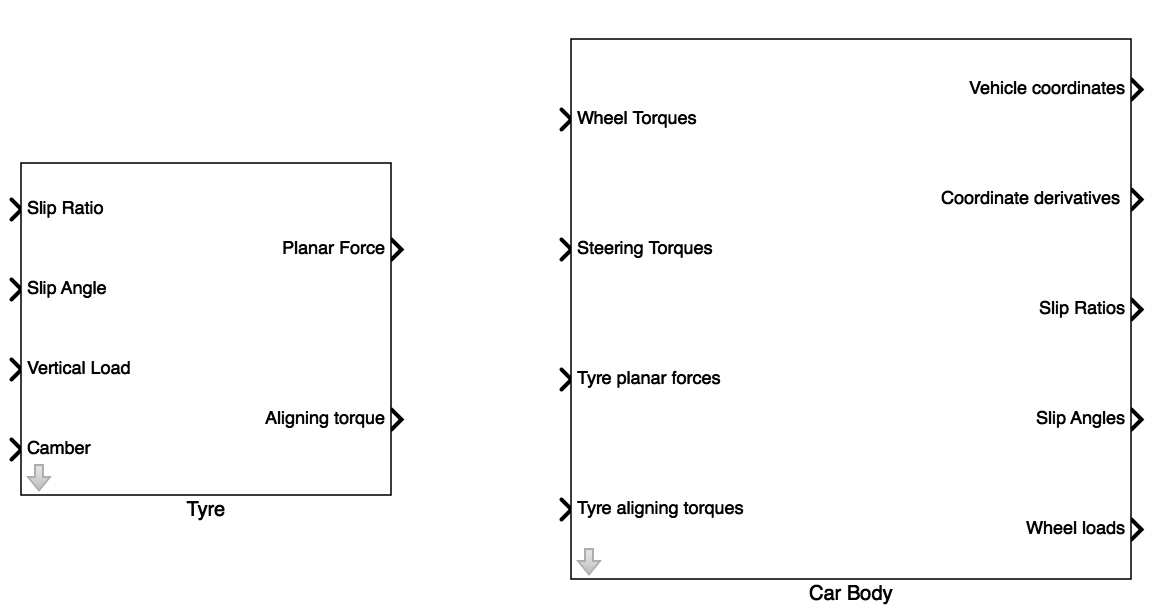
\includegraphics[scale=0.5]{images/bodyblockmask.png}
    \caption{Simulink blocks containing the tyre model and the 12DoF model.}
    \label{blocks}
\end{figure}

\section{Tyre block}

The Tyre model is implemented as a MATLAB function. The inputs are the slip ratio, the slip angle, the vertical force and the camber angle. The outputs are the horizontal force 2D vector $(F_x, F_y)$ and the aligning torque.
If all the tyres of the car are the same a single tyre block can be used to model all four wheels of the car, this is done by concantenating the inputs horizontally into a matrix. The forces corresponding to each tyre can then be extracted as columns of the outputs.
The outputs are computed by evaluating the Magic Formula equations described in \cite{pac2002}.
The coefficients representing the tyre for the simulations must be given in the Adams Car ".TIR" format. The format is human readable as a plaintext file, as described in \cite{pac2002}.
The tire model file must be located in the Matlab working directory. The name of the file can be entered in the "block mask" accessible by double clicking the block (Figure \ref{tyremask}).

\begin{figure}[ht]
    \centering
    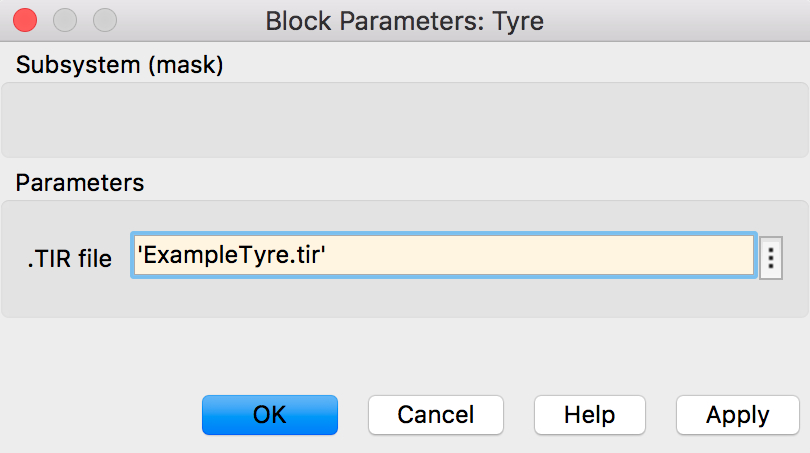
\includegraphics[scale=0.5]{images/tyremask.png}
    \caption{Simulink mask for the tyre block allows selection of the tyre model.}
    \label{tyremask}
\end{figure}

The parameters are loaded from the file into the tyre block workspace during the initialization phase by means of a script which takes advantage of the "loadTIR" function\cite{loadtir}.

Note that tyres are not always simmetrical. The model used in these simulations reflects this property and yields non-zero lateral force at zero slip angle. For this reason care should be taken when modelling tyres on opposite sides of the car. The ".TIR" files contain a field specifying for which side the empirical coefficients were fitted. To model tyres on the other side all inputs and outputs can be redefined in a simmetrical reference system. This simply means the slip angle and camber angle signs have to be changed before entering the tyre model and the lateral force and aligning moment signs have to be changed after they are output.

\section{Vehicle Body Block}
\label{sec:bodyblock}
The internal block diagram for the 12 DoF Model is shown in figure \ref{12diag}.
\begin{figure}[ht]
    \centering
    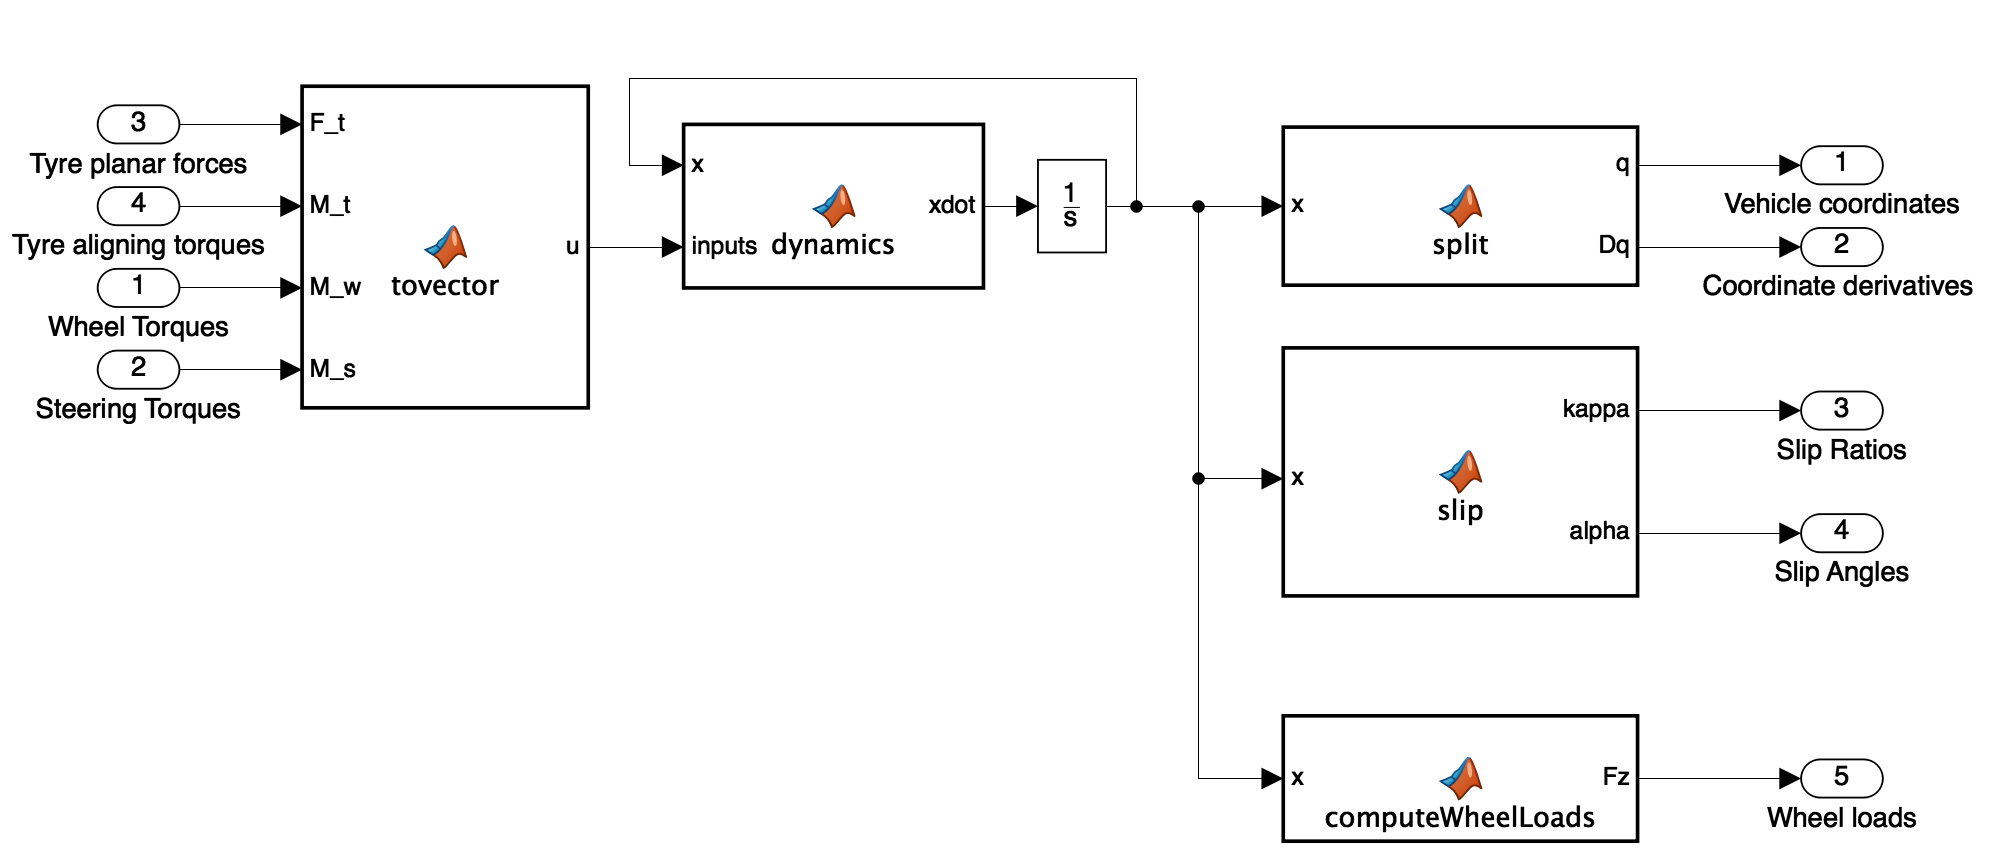
\includegraphics[width=\textwidth]{images/12dofinside.png}
    \caption{Simulink block diagram for the 12DoF model.}
    \label{12diag}
\end{figure}
The \textit{dynamics} block employs the state space representation of the system to evaluate the state derivative $\dot x$ from the state and the inputs. The state derivative, $\dot x$, is then integrated to close the physical feedback loop. The expressions used by the \textit{dynamics} block are loaded from a MATLAB function file created by the \textit{carmodel.m} script (Appendix \ref{sec:12dofcode}) discussed in section \ref{scriptdescription}.
The \textit{tovector} block simply assembles the incoming signals into the input vector for the dynamic system. The \textit{split} block disassembles the state vector $x$ into the lagragian coordinates and their derivatives.
The \textit{slip} block takes the vehicle coordinates as an input, calculates the contact point velocities and returns the slip angles and slip ratios.
The \textit{computeWheelLoads} block evaluates the vertical wheel forces using the formulas in section \ref{sec:6dofout}.

\subsection{Parameters and initial state}
The initial state for the integrator and the vehicle body parameters are taken from text files. The text files are in the format shown in figures \ref{params} and \ref{init}.
The file names are entered in the block mask as seen in Appendix \ref{chap:params}.

\begin{figure}[ht]
    \centering
    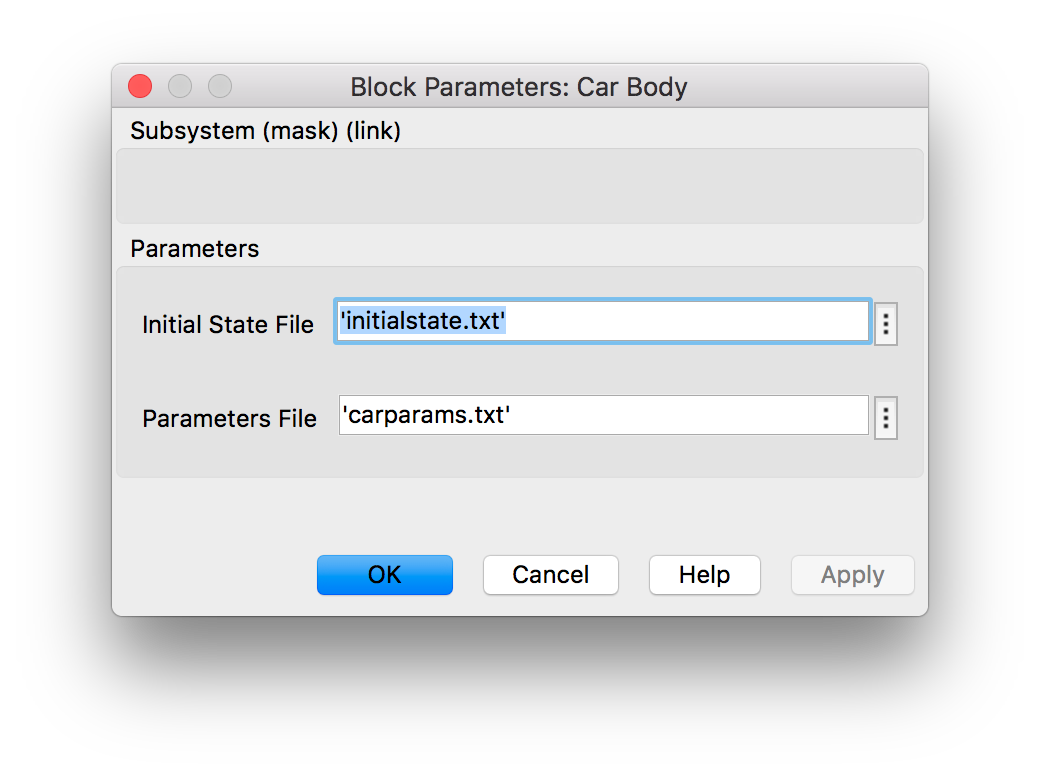
\includegraphics[scale=0.5]{images/bodymask.png}
    \caption{Simulink mask for the body dynamics block.}
	\label{12mask}
\end{figure}

\section{Mathematical model implementation script}
\label{scriptdescription}

Appendix \ref{sec:12dofcode} contains the full MATLAB script for the construction of the Lagrange equations of the 12DoF model and their solution.
The script is based on the symbolic math toolbox.

The script begins by defining symbols for vehicle parameters and inputs. Lagrangian coordinates and the necessary derivatives are declared as symbolic functions of the time variable \texttt{t}. Several groupings of these variables are made into one dimensional vectors. An example is given by \texttt{q} and \texttt{Dq} which respectively list symbols for the lagrangian coordinates and their first order derivatives.

The rotation matrices and CoG coordinates vector are defined to help in the coordinate transformations between inertial, undercarriage and chassis reference systems.
Matrices are also defined to rotate wheel forces and velocities from the wheel frames to the undercarriage frame.

Geometric points, velocities, forces and other three dimensional physical entities are expressed as column vectors of cartesian coordinates with respect to some reference system, explicited in the source code comments.

Lengthy code repetitions were avoided by taking advantage of the properties of matrix multiplication.
When dealing with the same quantity for each wheel of the car, such as the suspension travels or contact points, variables are grouped as columns of matrices. The order used is \texttt{FR - FL - RR - RL}. The following code snippet is provided as an example.

\lstinputlisting[firstnumber=118,firstline=118,lastline=123]{code/carmodel.m}

Here \texttt{p\_CG} is the CoG coordinates vector with respect to the inertial reference frame and \texttt{R} is the active rotation matrix from chassis to body frame.

When using the \texttt{diff()} function to differentiate the lagrangian coordinates with respect to time, the symbolic math toolbox uses place-holders such as \texttt{diff(x\_CG,t)}. These expressions are replaced by the script with the specifically defined symbols for the coordinate derivatives.

The \texttt{subs(expr, diff(q,t), Dq)} instruction is used to re-format the \texttt{expr} function containing time derivatives as it efficiently handles all the place-holders at once.

The function listed in appendix \ref{sec:genforces} uses the virtual work principle\cite{demeio} to find the generalized forces, $Q_i$ for the lagrangian formulation of the system.

The kinetic and potential energies, $T$ and $U$, are calculated and kept separate. The Langrangian is defined as
$$L = T - U$$
The Lagrange equations are given by evaluating
$$ \frac{d}{dt}\frac{\partial L}{\partial \dot q_i} - \frac{\partial L}{\partial q_i} + \frac{\partial D}{\partial \dot q_i}= Q_i$$
where $q_i$ takes the values of each of the lagrangian coordinates.
These equations may be written in the form

$$ \frac{d}{dt}\frac{\partial T}{\partial \dot q_i} = \frac{d}{dt}\frac{\partial U}{\partial \dot q_i} + \frac{\partial T}{\partial q_i} - \frac{\partial U}{\partial q_i} - \frac{\partial D}{\partial \dot q_i} + Q_i$$

Second order derivatives of the lagrangian coordinates can only occur in the left terms. Placeholders are initially used for the right hand sides.
Solving the resulting linear system of equations to find the second order derivatives is done using the \texttt{solve()} function. The right hand sides of the equations are then evaluated and substituted to the placeholders in the solutions.

The lagrangian coordinates and their first order derivatives constitute the vehicle state. The state space representation is assembled accordingly

The \texttt{matlabFunction()} command is used to save the system laws of motion to a file, to be executed by the simulink blocks. The same is done for the outputs of the model.

\begin{sidewaysfigure}[p]
    \centering
    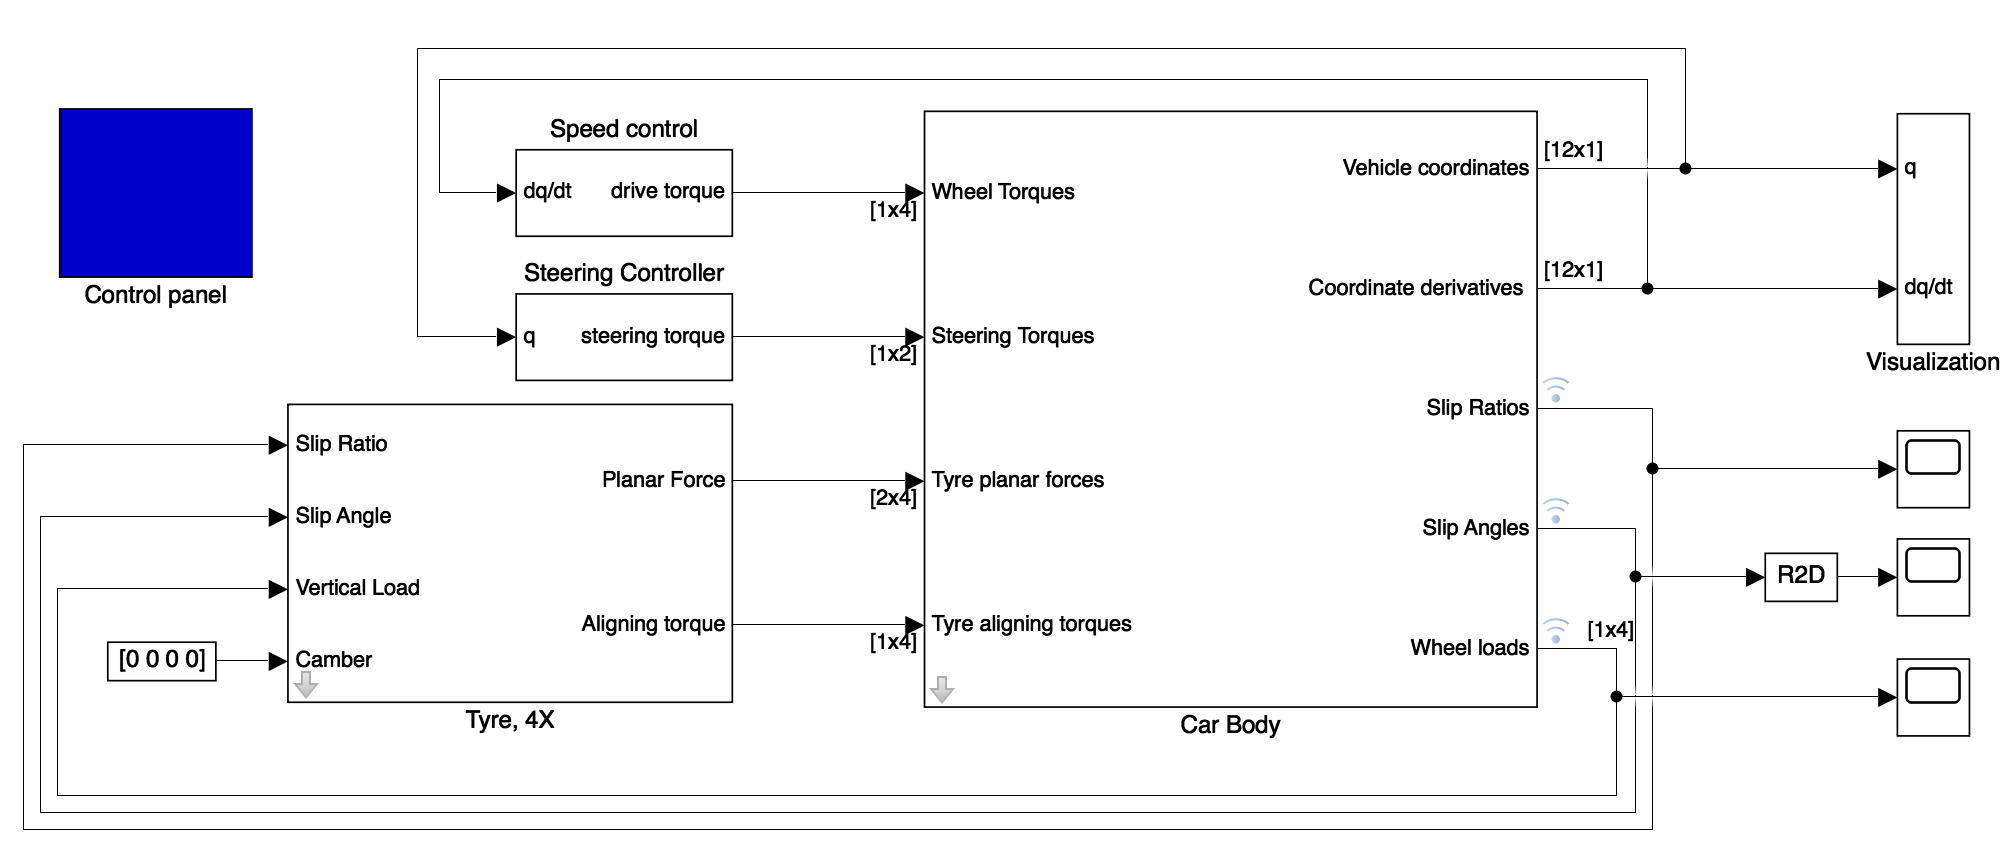
\includegraphics[width=\textwidth]{images/12doftest.png}
    \caption{Block diagram with steering and speed controllers for test simulations.}
    \label{12doftest}
\end{sidewaysfigure}

\section{The simulation configuration}
To obtain interesting data from a vehicle dynamics simulation the car model needs to receive a realistic input. Inputs for testing the discussed model were generated in different ways.

The first tests were done without the intervention of the tyre model. Constant forces or torques were directly applied to the model inputs to verify the expected behaviour.
After debugging the vehicle body model using this method the tyre model was connected, the resulting block diagram for the 12 DoF model is as shown in figure \ref{12doftest}.

The steering and speed controllers may be implemented in various ways to obtain the desired test conditions.

The \textit{visualization} subsystem includes several \textit{scope} blocks to plot interesting data such as the vehicle state, lateral accelerations, velocities, slip angles and more. The \textit{visualization} subsystem also contains a 2D animation feature adapted from \cite{animation}, shown in figure \ref{animfig}.

\begin{figure}[htb]
    \centering
    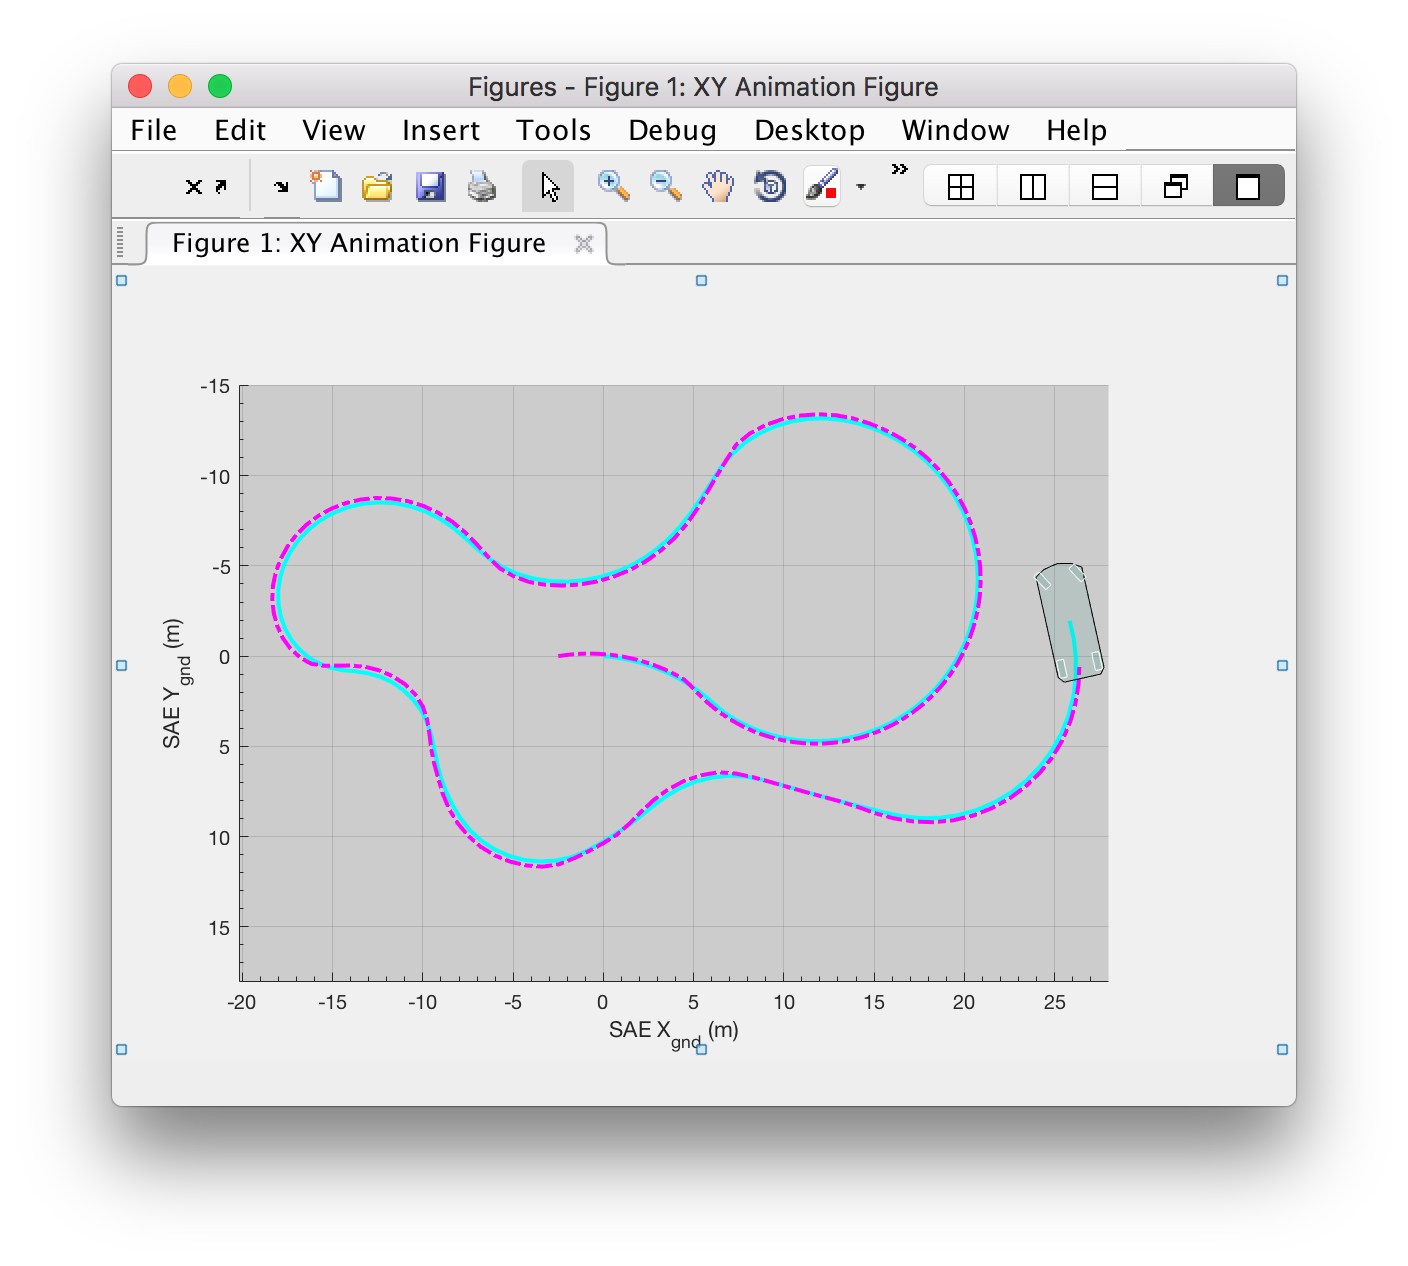
\includegraphics[scale=0.5]{images/2danimation.png}
    \caption{Simulink real time interface.}
	\label{animfig}
\end{figure}

\begin{figure}[h]
  \centering
  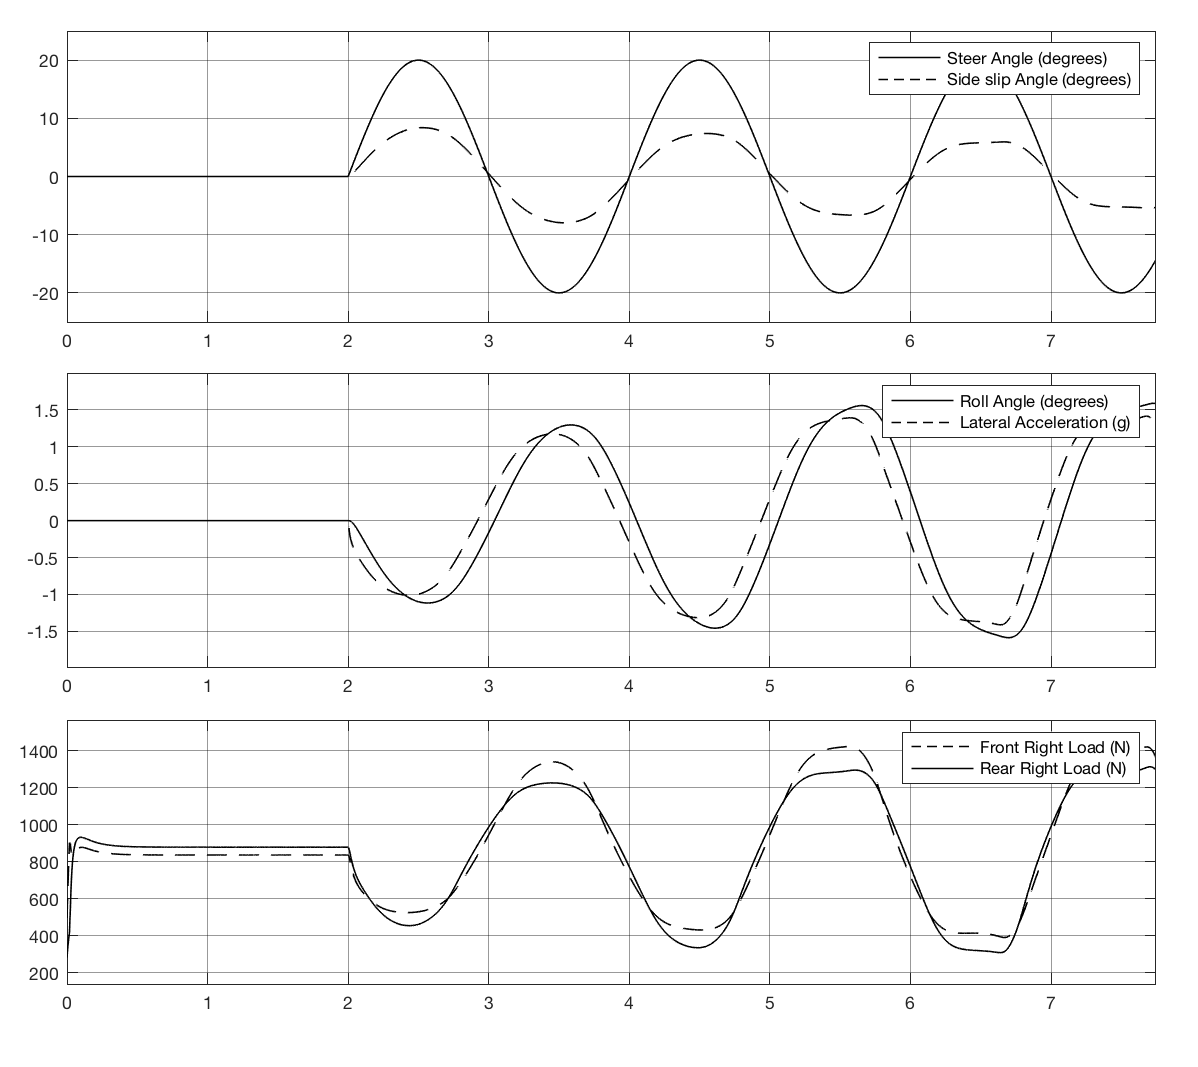
\includegraphics[scale=0.7]{figures/sine}
  \caption{Vehicle response for 0.5 Hz sinusoidal steering input.}
  \label{sine}
  \centering
  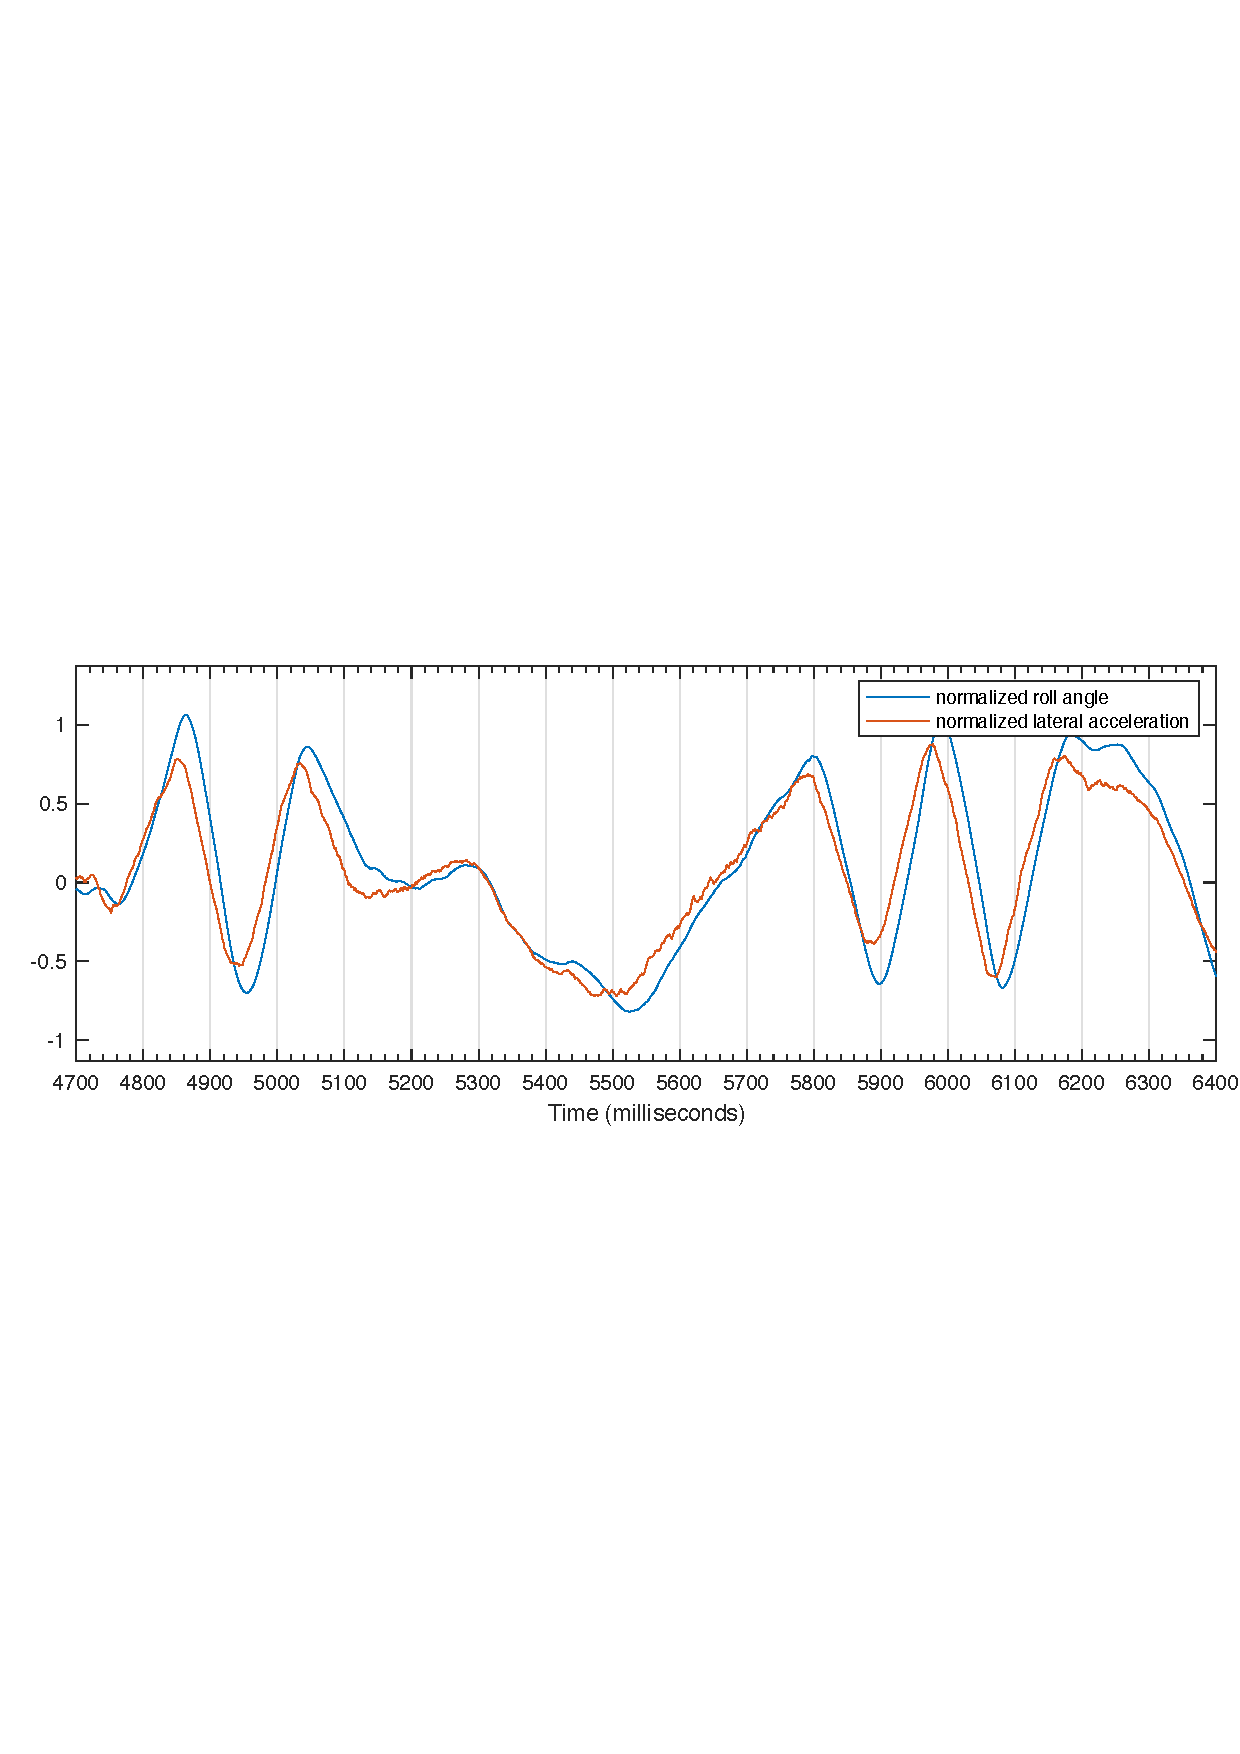
\includegraphics[scale=0.6]{figures/telemetry}
  \caption{Roll angle and lateral acceleration during slalom tests. The vehicle was driven twice through the same 5 cone slalom, completing a U-turn in between. [Data courtesy of Polimarche Racing Team]}
  \label{slalom}
\end{figure}

\subsection{Sinusoidal Steering Input}
A sinusoidal steering angle input was used to observe transients in the 6DoF vehicle model. Data resulting from this test is shown in figure \ref{sine}. Various phase delays can be observed between the most important physical quantities involved in handling dynamics, including load transfer and side slip angle. The side slip angle is defined as the angle between the undercarriage $x$ axis and the vehicle horizontal velocity $v_u = (\dot x_{CG}, \dot y_{CG}, 0)$. The delay between the roll angle and lateral acceleration is comparable to real experimental data captured during a slalom test, shown in figure \ref{slalom}. The test was run using the Peacock3 FSAE car built by Polimarche Racing Team.

\subsection{Manual steering and acceleration}
Simulink offers the possiblity to slow down simulations to real-time speed and
graphical user interface block to modify simulation parameters during execution. These two features in combination with the 2D animation shown in figure \ref{animfig} made it possible to manually drive the simulink model using the computer cursor, like a rudimentary videogame, whilst saving simulation data. The "driver" interface is shown in figure \ref{12mask}.

\begin{figure}[h]
    \centering
    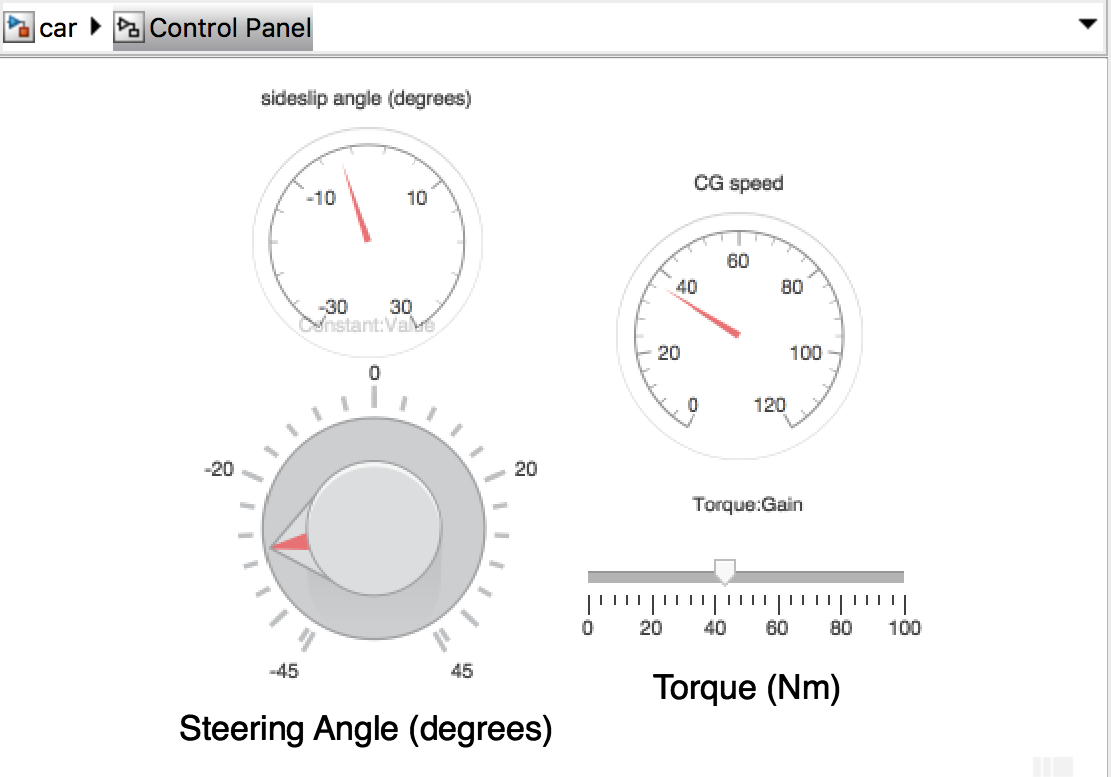
\includegraphics[scale=0.5]{images/controlpanel.png}
    \caption{Simulink real time interface for the 6DoF model.}
	\label{12mask}
\end{figure}


\subsection{Skidpad test}
A skidpad test consists in driving the examined vehicle in a circle with constant radius and at constant speed. This kind of test is easy to reproduce experimentally and is thus useful when validating vehicle dynamics models.

Maintaining constant speed is done by using a PID controller whose output is the torque equally applied to the rear wheels.

Following a circular trajectory can be seen as holding a constant distance from the origin of the inertial reference system. This was accomplished by using two controllers.

The first PID controller acts in a servo loop to hold a target steering angle.
Note that this controller is not needed in the 6DoF model as the steering angle does not have dynamics of its own.

The second PID controller generates the target steering angle to hold the desired distance from the reference point.
